%TeX

\section{Getting the flag}

\subsection{Recap}

\begin{frame}{A quick recap\ldots}
    \begin{columns}
        \column{0.5\textwidth}
        \begin{itemize}
            \item<1-> We have an x86 boot sector that's asking us for the flag
            \item<2-> The flag is clearly in the boot sector SOMEWHERE\ldots
            \begin{itemize}
                \item<3-> \ldots but not in plaintext, because this is a 400
                          point challenge and that would be too easy
            \end{itemize}
            \item<4-> So, where is it?
        \end{itemize}
        \column{0.5\textwidth}
        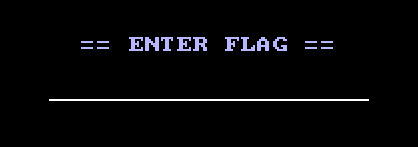
\includegraphics[width=\textwidth]{enter-flag}
    \end{columns}
\end{frame}

\begin{frame}{Reversing the boot sector}
    \begin{columns}
        \column{0.5\textwidth}
        \begin{itemize}
            \item<1-> Open the file in your favorite disassembler (e.g. IDA);
                      rebase at \texttt{0x7c00}
            \item<2-> We can visally pick out three sections:
            \begin{itemize}
                \item<2-> Init code (responsible for the protected
                          mode transition)
                \item<2-> Display code (identifiable by a large number of
                          \texttt{int} instructions)
                \item<2-> Some other code that uses Intel SSE2 instructions
            \end{itemize}
        \end{itemize}
        \column{0.5\textwidth}
        \begin{tikzpicture}
            \only<1> {\node (cfg) {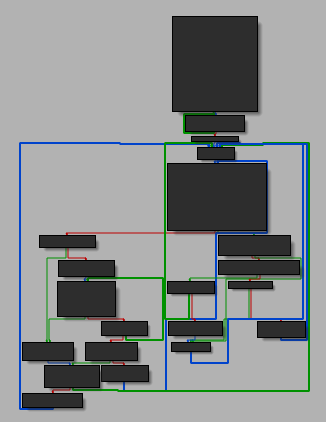
\includegraphics[width=\textwidth]{cfg}};}
            \uncover<2-> {\node (cfga) 
                {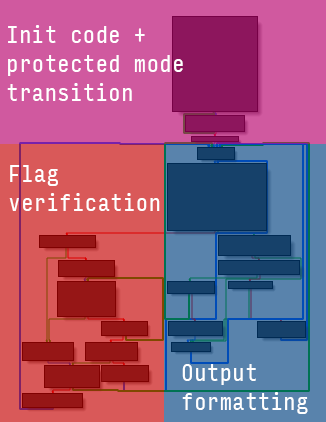
\includegraphics[width=\textwidth]{cfg-annotated}};}
        \end{tikzpicture}
    \end{columns}
\end{frame}

\subsection{First leads}

\begin{frame}{First leads}
    \begin{itemize}
        \item<1-> The program asks you to enter 20 characters, and immediately
                  breaks out if the first 4 characters aren't 'flag' after you
                  enter character \#20
        \item<2-> We can verify this in a debugger after eyeballing the code

        \begin{center}
            \uncover<3-> {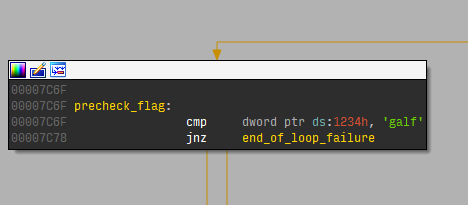
\includegraphics[width=0.7\textwidth]{flag-precheck}}
        \end{center}
    \end{itemize}
\end{frame}

\begin{frame}{As it turns out\ldots}
    \framesubtitle{After several hours of staring at x86 assembly}

    \begin{itemize}
        \item<1-> The flag is \alert{hashed} using a \alert{custom algorithm}
                  implemented with Intel SSE instructions (and this isn't very
                  surprising)
        \item<2-> {\em Ugh\ldots}
        \item<3-> We have to find an input to the hash algorithm that hashes
                  to the same value that's stored in the boot sector
    \end{itemize}
\end{frame}

\subsection{Diving into x86 instructions}

\begin{frame}{Suddenly, SSE2 instructions}
    \framesubtitle{``My Intel CPU can do {\em that?}''}
    The author of the challenge decided to use a bunch of obscure x86 SSE2
    instructions to force us to trawl through Intel documentation

    \begin{itemize}
        \item<2-> movaps\uncover<3->{: Moves to/from/between XMM registers}
        \item<2-> \alert<4->{andps}\uncover<3->{: Performs bitwise AND between
                                                XMM registers}
        \item<2-> pshufd\uncover<3->{: Reorders 32-bit words in XMM registers}
        \item<2-> \alert<4->{psadbw}\uncover<3->{: Sums absolute values of
                                                 differences between bytes
                                                 (it's as crazy as it sounds)}
    \end{itemize}

    \begin{block}<1->{Note}
        SSE2 instructions operate on XMM registers, which are 128 bits
        (16 bytes) wide.
    \end{block}

    \begin{alertblock}<4>{Question}
        Why are these instructions useful for writing a hash function (even if
        it's a bad hash function that we can break?)
    \end{alertblock}
\end{frame}

\newcommand{\StartCell}[2]{
    \node at (0,0) (#1) {\texttt{#2}};%
}
\newcommand{\Cell}[3]{
    \node [anchor=west] at (#1.east) (#2) {\texttt{#3}};%
}

\newcommand{\Xmm}[2]{%
    \getargsC{#2}%
    \raisebox{0.5em}{\texttt{xmm#1}:\xspace}%
    \begin{tikzpicture}[%
        every node/.style={%
            minimum width=1.5em,
            minimum height=0.75em,
            text height=0.75em,
            text depth=0.25em,
            outer sep=0pt,
            draw=black,
            semithick
        }
    ]%
        \StartCell{A}{\argi}%
        \Cell{A}{B}{\argii}%
        \Cell{B}{C}{\argiii}%
        \Cell{C}{D}{\argiv}%
        \Cell{D}{E}{\argv}%
        \Cell{E}{F}{\argvi}%
        \Cell{F}{G}{\argvii}%
        \Cell{G}{H}{\argviii}%
        \Cell{H}{I}{\argix}%
        \Cell{I}{J}{\argx}%
        \Cell{J}{K}{\argxi}%
        \Cell{K}{L}{\argxii}%
        \Cell{L}{M}{\argxiii}%
        \Cell{M}{N}{\argxiv}%
        \Cell{N}{O}{\argxv}%
        \Cell{O}{P}{\argxvi}%
    \end{tikzpicture}%
}

\newcommand{\Left}[2]{\textcolor<#2>{red}{#1}}

\newcommand{\Right}[2]{\textcolor<#2>{orange}{#1}}

\newcommand{\PsadbwIllustration}[5]{
    \visible<#1>{\Xmm{0}{0 1 2 3 4 5 6 7 8 9 10 11 12 13 14 15}} \\
    \visible<#2>{
        \raisebox{0.3em}{\scriptsize\em (minus)} \\
        \Xmm{1}{15 14 13 12 11 10 9 8 7 6 5 4 3 2 1 0} \\
    }
    \visible<#3>{
        \raisebox{0.3em}{\scriptsize $\downarrow$} \\
        \Xmm{0}{-15 -13 -11 -9 -7 -5 -3 -1 1 3 5 7 9 11 13 15} \\
    }
    \visible<#4>{
        \raisebox{0.3em}{\scriptsize\em (absolute values)} \\
        \Xmm{0}{%
            \Left{15}{#5}
            \Left{13}{#5}
            \Left{11}{#5}
            \Left{9}{#5}
            \Left{7}{#5}
            \Left{5}{#5}
            \Left{3}{#5}
            \Left{1}{#5}
            \Right{1}{#5}
            \Right{3}{#5}
            \Right{5}{#5}
            \Right{7}{#5}
            \Right{9}{#5}
            \Right{11}{#5}
            \Right{13}{#5}
            \Right{15}{#5}
        } \\
    }
    \visible<#5>{
        \raisebox{0.3em}{\scriptsize\em (16-bit sums)} \\
        \Xmm{0}{%
            0 0 0 0 0 0 \Left{64}{#5} \Left{0}{#5} 0 0 0 0 0 0 \Right{64}{#5} \Right{0}{#5}
        } \\
    }
}

\begin{frame}{Packed Sum of Absolute Differences of Bytes in Word}
    \framesubtitle{That's a mouthful\ldots}
    \begin{center}
        \PsadbwIllustration{1-}{2-}{3-}{4-}{5-}
        \pause \pause \pause \pause \pause
        \begin{alertblock}{It's hard to go back\ldots}
            If you just have the result, you have to find two sets of eight
            bytes where the absolute values of their differences sum to 64
            (and there are many)
        \end{alertblock}
    \end{center}
\end{frame}

\newcounter{SudokuRowCount}
\newcounter{SudokuColCount}
\newcounter{SudokuColIndex}
\newcommand{\SudokuRow}[1]{%
    \setcounter{SudokuColIndex}{0}%
    \setcounter{SudokuColCount}{1}%
    \getargsC{#1}%
    \whiledo{\value{SudokuColIndex} < \narg}{%
        \pgfmathparse{\value{SudokuColCount} - 0.5}%
        \edef\x{\pgfmathresult}%
        \pgfmathparse{\SudokuSize + 0.5 - \value{SudokuRowCount}}%
        \edef\y{\pgfmathresult}%
        \stepcounter{SudokuColIndex}%
        \edef\n{\csname arg\roman{SudokuColIndex}\endcsname}%
        \node[anchor=center] at (\x, \y) {\texttt{\n}};%
        \stepcounter{SudokuColCount}%
    }%
    \stepcounter{SudokuRowCount}%
}

\NewEnviron{sudoku}[2]{%
    \begin{tikzpicture}[
        scale=#2,
        every node/.style={%
            text depth=-0.75ex,
            text height=0.5ex
        }
    ]%
        \pgfmathsetmacro{\SudokuSize}{pow(#1, 2)}%
        \draw (0, 0) grid (\SudokuSize, \SudokuSize);%
        \draw[very thick, scale=#1] (0, 0) grid (#1, #1);%
        \setcounter{SudokuRowCount}{1}%
        \BODY
    \end{tikzpicture}%
}

\newcommand{\DefconSudoku}[2]{%
    \begin{sudoku}{4}{#2}
        \SudokuRow{\alert<#1>{d} \alert<#1>{c} \alert<#1>{6} \alert<#1>{1} \alert<#1>{9} 0 e b 5 7 3 2 4 8 f a}
        \SudokuRow{5 8 a 4 f c 2 d 9 0 b e 3 7 6 1}
        \SudokuRow{2 b 9 7 5 3 6 1 4 8 a f d 0 e c}
        \SudokuRow{0 3 f e 4 a 8 7 \alert<#1>{d} \alert<#1>{c} \alert<#1>{6} \alert<#1>{1} \alert<#1>{9} b 2 5}
        \SudokuRow{8 \alert<#1>{d} \alert<#1>{c} \alert<#1>{6} \alert<#1>{1} \alert<#1>{9} 3 2 b 5 e 7 0 4 a f}
        \SudokuRow{b 1 5 0 d 8 c 6 f a 9 4 7 2 3 e}
        \SudokuRow{9 a 4 f 7 5 0 e 2 3 1 8 b d c 6}
        \SudokuRow{7 2 e 3 b 4 a f 0 \alert<#1>{d} \alert<#1>{c} \alert<#1>{6} \alert<#1>{1} \alert<#1>{9} 5 8}
        \SudokuRow{e 4 \alert<#1>{d} \alert<#1>{c} \alert<#1>{6} \alert<#1>{1} \alert<#1>{9} 0 a b 2 5 8 f 7 3}
        \SudokuRow{1 9 8 2 3 7 5 4 e 6 f 0 a c d b}
        \SudokuRow{f 6 7 a 2 d b c 1 9 8 3 5 e 0 4}
        \SudokuRow{3 5 0 b a e f 8 7 4 \alert<#1>{d} \alert<#1>{c} \alert<#1>{6} \alert<#1>{1} \alert<#1>{9} 2}
        \SudokuRow{a e 3 \alert<#1>{d} \alert<#1>{c} \alert<#1>{6} \alert<#1>{1} \alert<#1>{9} 8 f 7 b 2 5 4 0}
        \SudokuRow{6 0 2 5 e b d 3 c 1 4 9 f a 8 7}
        \SudokuRow{c 7 1 9 8 f 4 5 6 2 0 a e 3 b d}
        \SudokuRow{4 f b 8 0 2 7 a 3 e 5 \alert<#1>{d} \alert<#1>{c} \alert<#1>{6} \alert<#1>{1} \alert<#1>{9}}
    \end{sudoku}
}

\subsection{Introduction to SMT solvers}

\begin{frame}{SAT solvers to the rescue!}
    \framesubtitle{How to master Sudoku without memorizing strategies}
    \begin{columns}
        \column{0.5\textwidth}
        {\em
            ``I think a serious case can be made that the decline in the
            American economy can be blamed on the sapping of the mental energy
            and productivity of the American workforce that sudoku addiction
            alone has wrought''
        } \\
        \begin{flushright}
            -- Some Slate writer \\
        \end{flushright}

        \uncover<2->{Notice anything strange about this puzzle?} \\
        \uncover<3->{Stranger still: a SAT solver created it from thin air}
        \column{0.5\textwidth}

        \uncover<2-> {\DefconSudoku{3-}{0.33}}
    \end{columns}
\end{frame}

\begin{frame}{What's a SAT (or SMT) solver?}
    \begin{itemize}
        \item<1-> SAT solvers
        \begin{itemize}
            \item<2-> Only operate on Boolean logic
            \item<3-> Take large sets of Boolean CNFs (e.g.
                  $(v_1 \lor v_2 \lor v_3) \land (v_4 \lor v_5 \lor v_6)$)
            \item<4-> Try to come up with inputs so the formula returns true
                  (or fail and report that the formula is ``unsatisfiable'',
                  which means that it's impossible for the formula to be true)
        \end{itemize}

        \item<5-> SMT solvers
        \begin{itemize}
            \item<6-> ``Satisfiability modulo theories'' - a fancy term for a
                      piece of software that uses a SAT solver to act as a
                      theorem prover
            \item<7-> Takes standard mathematical operations, bit operations,
                      etc, and converts them to Boolean CNFs that a SAT solver
                      can work with
            \item<8-> Again, tries to come up with inputs so that the formula
                      is satisfiable
        \end{itemize}

        \item<9-> Symbolic execution engines
        \begin{itemize}
            \item<10-> Convert CPU instructions into a SMT solver language
        \end{itemize}
    \end{itemize}
\end{frame}

\begin{frame}{In case this all seemed too abstract\ldots}
    \begin{center}
        {\Large
            SMT solvers let you write a type of SQL \alert{that
            can be used to solve certain hard\textsuperscript{*} problems}
        } \pause \\
        * hard, meaning ``NP-complete'' \pause \\
        \vspace{0.25in}
        {\Large
            The SMT query itself can be constructed from a language like
            Python, C, or even raw x86 assembly
        } \pause \\
        \vspace{0.25in}
        {\Large
            If there's one thing you should take from this presentation:
            SMT solvers are tools for solving constraint problems, just like
            SQL is a tool for making sense of large amounts of data
        }
    \end{center}
\end{frame}

\begin{frame}{Modern SMT solvers and symbolic execution engines}
    \begin{itemize}
        \item<1-> \alert<4->{Z3} (SMT)
        \begin{itemize}
            \item<1-> Open source, developed by Microsoft
            \item<1-> Has its own SQL-like language, with Python bindings
            \item<1-> Contains its own SAT solver
        \end{itemize}
        \item<2-> KLEE (symbolic execution)
        \begin{itemize}
            \item<2-> Used to instrument code that can be recompiled to LLVM IR
            \item<2-> C bindings
            \item<2-> Z3, Kleaver, or SMTLib used as a backend
        \end{itemize}
        \item<3-> Ponce (symbolic execution)
        \begin{itemize}
            \item<3-> An IDA Pro plugin for x86 and x86\_64 instruction sets
            \item<3-> Z3 used as a backend
        \end{itemize}
    \end{itemize}

    \visible<4->{
        We'll be mainly focusing on using Z3, since all the other tools use it
        under the hood (and it's awesome)
    }
\end{frame}

\newcommand{\PythonBox}[2]{%
    {%
        \setbeamercolor{block body}{bg=black!100,fg=white}
        \setbeamercolor{block title}{bg=black!70,fg=white}
        \begin{block}{#1}%
            {
                \inputminted[
                    style=monokai
                ]{py}{include/code/#2.py}%
            }%
        \end{block}%
    }%
}

\subsection{Generating sudoku puzzles}

\begin{frame}{Back to our sudoku\ldots}
    How do you create a hexadoku puzzle out of thin air with Z3? \pause \\

    \PythonBox{Creating the board}{01-declare-board}
\end{frame}

\begin{frame}{Telling z3 how to play sudoku}
    We'll define our first rule: each cell has to be between 0 and 15 \pause \\

    \PythonBox{The most basic of Sudoku rules}{02-number-range}
\end{frame}

\begin{frame}{Telling z3 how to play sudoku}
    Now, the rules everyone knows \pause \\

    \PythonBox{Rows and columns}{03-uniques}
\end{frame}

\begin{frame}{Telling z3 how to play sudoku}
    Mini-boxes are slightly more complicated \pause \\

    \PythonBox{Mini-boxes}{04-mini-boxes}
\end{frame}

\begin{frame}{Telling z3 how to play {\em our version of} sudoku}
    Now for the initial values \\
    \ldots\xspace dc858 isn't sudoku-able, but dc619 is \pause \\

    \PythonBox{Initial values}{05-initial}
\end{frame}

\begin{frame}{Telling z3 to start solving}
    This will take a little bit of time \pause \\

    \PythonBox{Start solving!}{06-start-solving}
\end{frame}

\begin{frame}{The results\ldots}
    \begin{center}
        \DefconSudoku{1-}{0.4}
    \end{center}
\end{frame}

\begin{frame}{The power of SMT solvers}
    \framesubtitle{Maybe familiar to anyone who's tried Prolog}
    \begin{center}
        {\Large
            We only had to \alert{define the constraints of the puzzle we
            wanted}, and Z3 found one satisfying those constraints
        }
    \end{center}
\end{frame}

\subsection{Translating x86 assembly to a SMT solver}

\begin{frame}{Constraint solving our boot sector}
    ``Hey, Z3, I want you to find me input values that, after being put through
    this crazy operation (among other things), end up being equal to the ones
    stored in the boot sector''
    \\
    \begin{center}
        \PsadbwIllustration{1-}{1-}{1-}{1-}{1-}
    \end{center}
\end{frame}

\begin{frame}{Useful primitives}
    \begin{itemize}
        \item We need to implement the pshufd and psadbw x86 instructions
              in Z3
        \item Documentation at \url{http://x86.renejeschke.de} already
              provides us pseudocode for these instructions
    \end{itemize}

    \begin{center}
        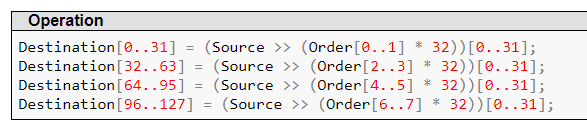
\includegraphics[width=0.75\textwidth]{pshufd-docs}
    \end{center}
\end{frame}

\begin{frame}{Useful constraints}
    The flag looks like \texttt{flag\{some\_text\_here\}}, but the
    word ``flag'' is chopped off before it's loaded into an XMM register,
    so the first and last characters of the remaining 16 are \texttt{\{} and
    \texttt{\}}, respectively \\ \pause

    This may not look like much, but we already have a few constraints\ldots

    \PythonBox{Initial constraints}{10-useful-constraints}
\end{frame}

\newcommand{\WA}[1]{%
    \textcolor{red}{#1}%
}

\newcommand{\WB}[1]{%
    \textcolor{blue}{#1}%
}

\newcommand{\WC}[1]{%
    \textcolor{orange}{#1}%
}

\newcommand{\WD}[1]{%
    \textcolor{magenta}{#1}%
}

\begin{frame}{Implementing the hash function's word shuffling}
    The flag is initially shuffled using the pshufd instruction; create a new
    constraint (``shuf'') that just describes the permutation \\ \pause

    \begin{center}
        \Xmm{0}{\WA{\{} \WA{A} \WA{B} \WA{C} \WB{D} \WB{E} \WB{F} \WB{G} \WC{H} \WC{I} \WC{J} \WC{K} \WD{L} \WD{M} \WD{N} \WD{\}}}
        \raisebox{0.3em}{\scriptsize $\downarrow$\xspace\texttt{pshufd xmm0, xmm0, 0x1e}} \\
        \Xmm{0}{\WC{H} \WC{I} \WC{J} \WC{K} \WD{L} \WD{M} \WD{N} \WD{\}} \WB{D} \WB{E} \WB{F} \WB{G} \WA{\{} \WA{A} \WA{B} \WA{C}}
    \end{center}
    \pause
    \PythonBox{Implementing the word shuffling (pshufd)}{11-pshufd}
\end{frame}

\begin{frame}{Implementing the hash function's bitmasking}
    For each of the hash function's 8 rounds, a different mask is applied to
    the shuffled value, so create another set of intermediate values called
    ``masked'' \\ \pause
    \PythonBox{Implementing the masking operation (andps)}{12-masking}
\end{frame}

\begin{frame}{Implementing the packed sum of absolute differences}
    A single x86 instruction turned into like 30 lines of Python\ldots \\
    \pause
    \PythonBox{Implementing psadbw (greatly simplified; trust me, it's nasty)}{13-psadbw}
\end{frame}

\begin{frame}{And the rest of the algorithm\ldots}
    \framesubtitle{AKA: continuing to give up on explaining the details}
    \begin{columns}
        \column{0.5\textwidth}

        \begin{itemize}
            \item Would be boring to present, since there were a few arbitrary
                  things thrown into the challenge that made it deliberately
                  more annoying to reverse-engineer
            \item \ldots\xspace Like x86 tricks where they loaded a register
                  like \texttt{eax} and used \texttt{ah} and \texttt{al}
                  backwards
            \item Not to mention that the algorithm has to run for 8
                  iterations\ldots
        \end{itemize}
        \column{0.5\textwidth}
        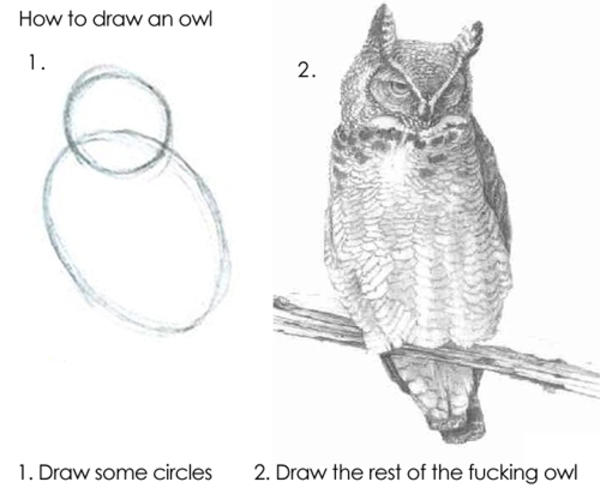
\includegraphics[width=\textwidth]{owl}
    \end{columns}
\end{frame}

\begin{frame}{Once we've got the constraints defined\ldots}
    Now, we can solve it as usual, and retrieve the flag from the model \\
    \pause
    \PythonBox{Solving for the flag}{14-start-solving}
\end{frame}

\begin{frame}{Run it, and\ldots}
    \begin{center}
        {\Large
            \texttt{Formula was satisfiable.} \\
            \texttt{flag\{ D`?T\textbackslash{}B?3F>~P`\}}
        }
    \end{center}
\end{frame}

\subsection{Debugging your keygen}

\begin{frame}{Does it work?}
    \begin{columns}
        \column{0.5\textwidth}
        Well, no

        \column{0.5\textwidth}
        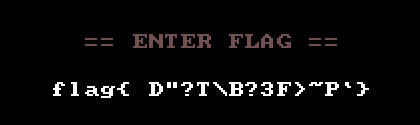
\includegraphics[width=\textwidth]{one-round-entry} \\
        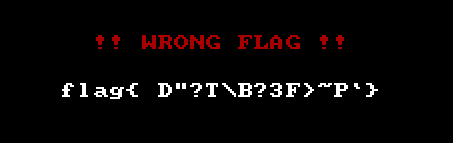
\includegraphics[width=\textwidth]{one-round-invalid}
    \end{columns}
\end{frame}

\begin{frame}{Does it work?}
    \begin{columns}
        \column{0.5\textwidth}
        But, using IDA's debugger and setting breakpoints, we see that it
        got through the first round of the hash function, but failed on the
        second - turns out, we forgot to solve the remaining rounds

        \column{0.5\textwidth}
        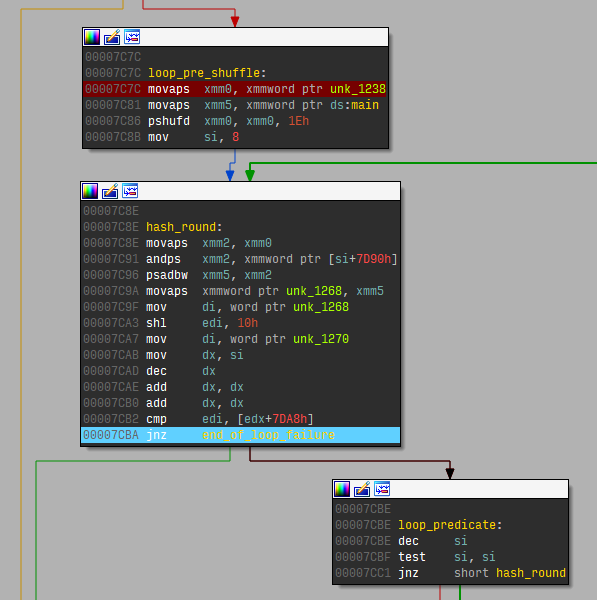
\includegraphics[width=\textwidth]{one-round-success}
    \end{columns}
\end{frame}

\begin{frame}{Debugging SMT solvers}
    \begin{itemize}
        \item<1-> Baby steps - try to get a satisfiable formula first, then
                  focus on making it the {\em correct} satisfiable formula
        \item<2-> If you're getting unsatisfiable, make sure you're not
                  overconstraining (i.e. assuming that the flag only contains
                  letters)
        \item<3-> If you're reimplementing some piece of code in Z3, make sure
                  its flow matches the original's
        \begin{itemize}
            \item<4-> Match control structures as faithfully as possible
            \item<5-> Use Python functions to implement complex behaviors like
                      Intel SSE2 instructions with the correct series of 
                      \texttt{smt.add} calls
        \end{itemize}
    \end{itemize}
\end{frame}

\begin{frame}{After some refactoring\ldots}
    \begin{center}
        {\Large
            \texttt{Formula was satisfiable.} \\
            \texttt{flag\{4e@alz\_p\%Z/TnW\}} \pause \\
            \vspace{0.5in}
            And, it got through 6 out of the 8 rounds this time! \pause \\
            \ldots\xspace But, it returned unsatisfiable when trying to solve
            for 7 or 8
        }
    \end{center}
\end{frame}

\begin{frame}{Typos are your worst enemy}
    \framesubtitle{Spot the difference\ldots}
    \begin{columns}
        \column{0.3\textwidth}
        \PythonBox{What I typed}{20-incorrect-constants}
        \column{0.1\textwidth}
        \column{0.6\textwidth}
        \PythonBox{What I meant}{21-correct-constants}
    \end{columns}
\end{frame}

\begin{frame}{After fixing the typo\ldots}
    \begin{center}
        {\Large
            \texttt{Formula was satisfiable.} \\
            \texttt{flag\{4r3alz\_m0d3\_y0\}} \\
        }
        \pause \vspace{0.5in}
        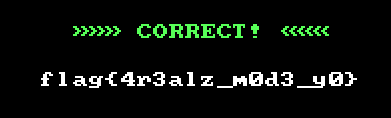
\includegraphics[width=0.75\textwidth]{flag-correct}
    \end{center}
\end{frame}

\begin{comment}
\begin{frame}{Irreversible transforms and hash functions}
    \framesubtitle{It's only sort of magic}
    \begin{itemize}
        \item<1-> Hash functions are usually defined as
                  $H(s, x) \rightarrow \{0, 1\}^\ell$, where $s$ is the 'seed',
                  $x$ is the message, and $\ell$ is some fixed number of bits
        \item<2-> The 'seed' is some public value used to initialize the hash
                  function's state
        \item<3-> There are a series of repeated 'reductions' meant to take the
                  message and perform some sort of irreversible transform on it
                  one block at a time
    \end{itemize}
    \begin{block}<4->{Example}
        For SHA256, $s$ is the fractional part of the cube roots of the first
        64 primes, $\ell = 256$, and the reductions involve a few non-linear
        functions (i.e. addition/XOR of multiple values, taking the majority of
        three bits, etc). The idea is that {\em you can't get the original
        message back once you start scrambling it.}
    \end{block}
\end{frame}
\end{comment}
